\chapter{Résultats Expérimentaux et Analyses Graphiques}
\label{chap:resultats}

Ce chapitre présente le protocole expérimental rigoureux mis en place et analyse les résultats comparatifs obtenus sur les problèmes continus et discrets à travers les visualisations graphiques et les données statistiques enregistrées.

\section{Protocole Expérimental et Métriques d'Évaluation}
Afin de garantir une reproductibilité parfaite et une rigueur méthodologique sans biais, toutes les expériences respectent les critères suivants :
\begin{itemize}[label=\textbullet]
    \item \textbf{Échantillonnage Monte Carlo :} 30 répétitions indépendantes pour chaque configuration d'algorithme (totalisant 120 exécutions complètes pour GWO/GT-GWO) ;
    \item \textbf{Contrôle des graines aléatoires :} les graines du générateur pseudo-aléatoire sont initialisées de façon déterministe ($\text{seed} = 42 + \text{run}$) et partagées rigoureusement entre algorithme classique et hybride pour chaque run apparié ;
    \item \textbf{Métriques statistiques calculées :} Meilleure valeur (Best), Pire valeur (Worst), Moyenne arithmétique (Mean), Écart-type (Std), Taux de succès à l'optimum global ($\%$) et Temps de calcul CPU moyen en secondes ;
    \item \textbf{Validation statistique :} Test de rang signé de Wilcoxon (\textit{Wilcoxon signed-rank test}) appliqué aux paires d'exécutions pour tester la significativité statistique ($p$-value).
\end{itemize}

% -----------------------------------------------------------------------------
\section{Expérimentation Continue : GWO vs GT-GWO sur Rastrigin}

\subsection{Présentation de la Fonction de Rastrigin}
La fonction de Rastrigin en dimension $d = 2$ est un benchmark continu hautement multimodal, caractérisé par un très grand nombre de minima locaux disposés selon un maillage régulier :
\begin{equation}
    f(\mathbf{x}) = 10d + \sum_{i=1}^d \left(x_i^2 - 10 \cos(2\pi x_i)\right), \qquad x_i \in [-5.12, 5.12]
\end{equation}
Son optimum global unique est situé en $\mathbf{x}^* = (0, \dots, 0)$ avec $f(\mathbf{x}^*) = 0$.

\subsection{Analyse Comparative des Performances Numériques}
Le tableau \ref{tab:rastrigin_summary} consigne les statistiques enregistrées sur les 30 runs indépendants (taille de population $N = 30$, budget de 100 itérations).

\begin{table}[h!]
    \centering
    \caption{Synthèse comparative sur la fonction continue de Rastrigin (30 runs)}
    \label{tab:rastrigin_summary}
    \small
    \begin{tabularx}{\textwidth}{lcccccc}
        \toprule
        \textbf{Algorithme} & \textbf{Best} & \textbf{Worst} & \textbf{Moyenne (Mean)} & \textbf{Écart-type (Std)} & \textbf{Succès} & \textbf{Temps (s)} \\
        \midrule
        GWO classique & $0.0000$ & $1.4792 \times 10^{-1}$ & $4.9305 \times 10^{-3}$ & $2.7006 \times 10^{-2}$ & 96.7\% & \textbf{0.2718} \\
        \textbf{GT-GWO (Hybride)} & \textbf{0.0000} & \textbf{0.0000} & \textbf{0.0000e+00} & \textbf{0.0000e+00} & \textbf{100.0\%} & 0.3621 \\
        \bottomrule
    \end{tabularx}
\end{table}

Comme l'atteste le tableau \ref{tab:rastrigin_summary}, le GWO classique échoue à converger dans $3.3\%$ des cas (run n$^\circ$10), où il reste bloqué dans un minimum local avec un fitness dégradé de $0.1479$. À l'inverse, \textbf{GT-GWO atteint un taux de succès parfait de 100.0\%} avec une moyenne et une variance strictement nulles ($0.0000 \pm 0.0000$), garantissant une robustesse absolue face aux pièges multimodaux.

\subsection{Analyses Graphiques : Convergence et Boîtes à Moustaches}
La figure \ref{fig:rastrigin_convergence} met en regard la dispersion des solutions et la courbe de convergence moyenne en échelle semi-logarithmique.

\begin{figure}[h!]
    \centering
    \begin{subfigure}[b]{0.48\textwidth}
        \centering
        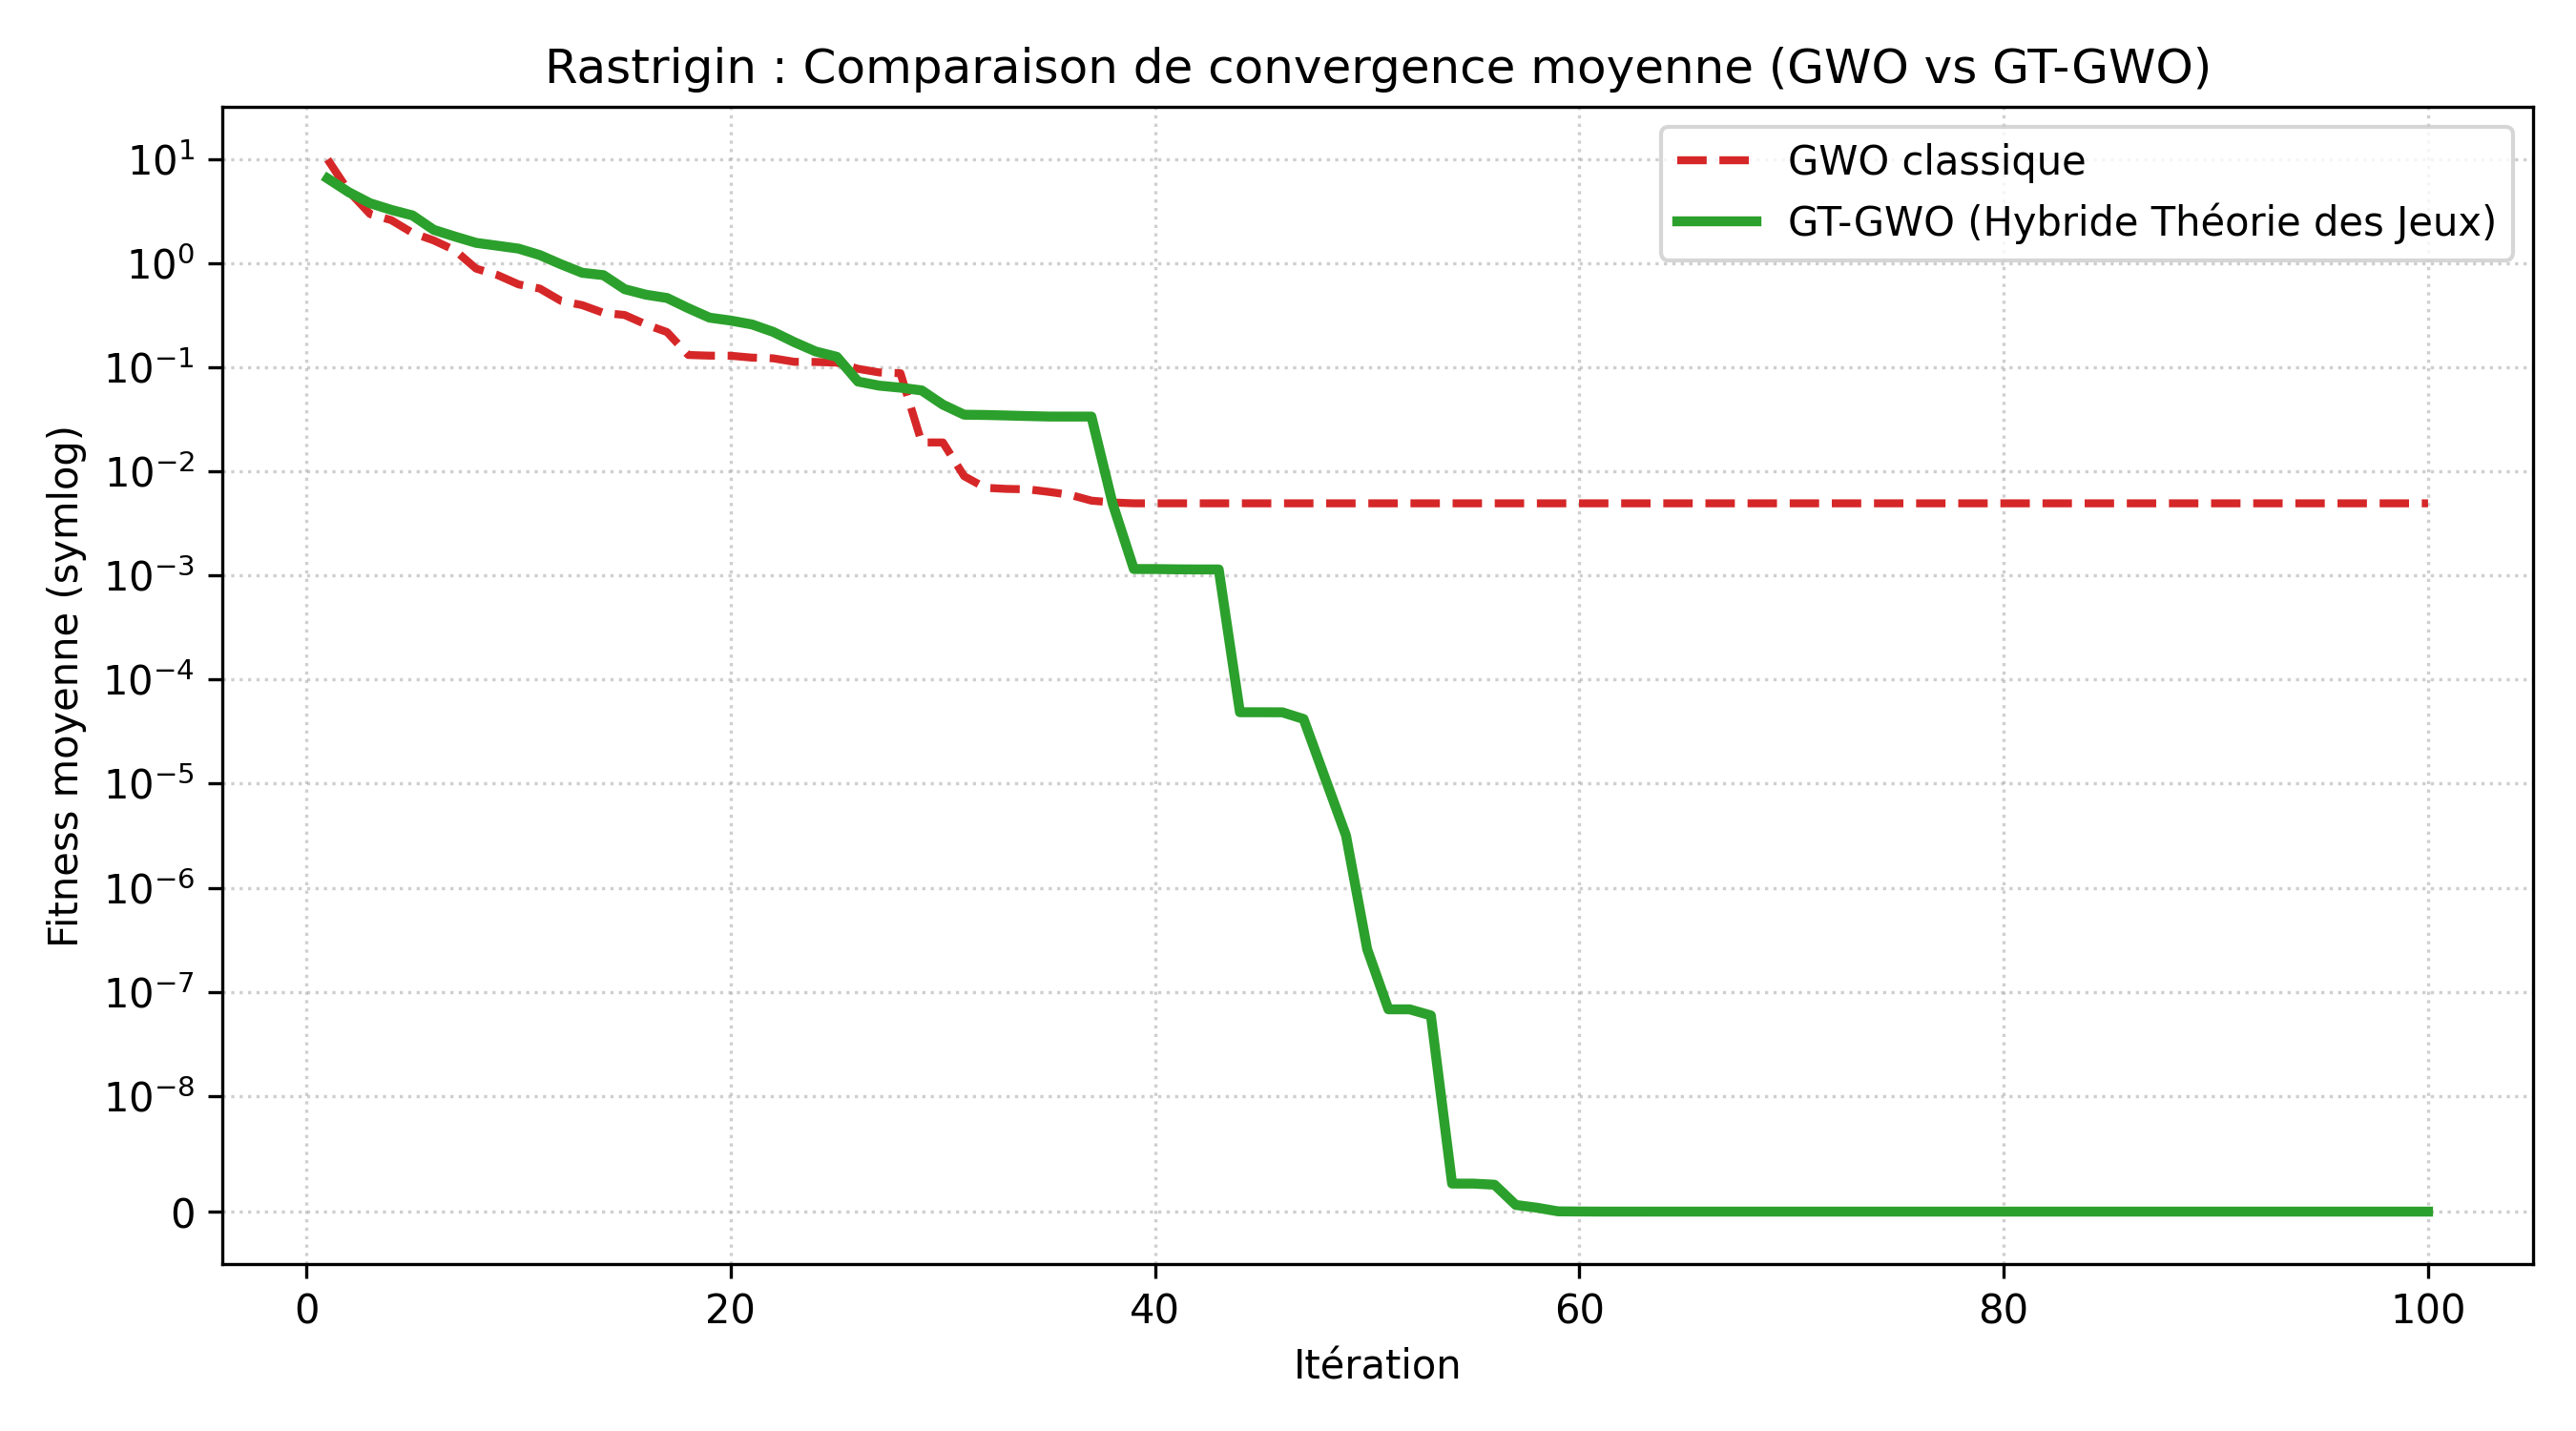
\includegraphics[width=\textwidth]{figures/comparison_rastrigin.png}
        \caption{Dispersion (Boxplot) et Fitness moyen}
        \label{fig:rastrigin_box}
    \end{subfigure}
    \hfill
    \begin{subfigure}[b]{0.48\textwidth}
        \centering
        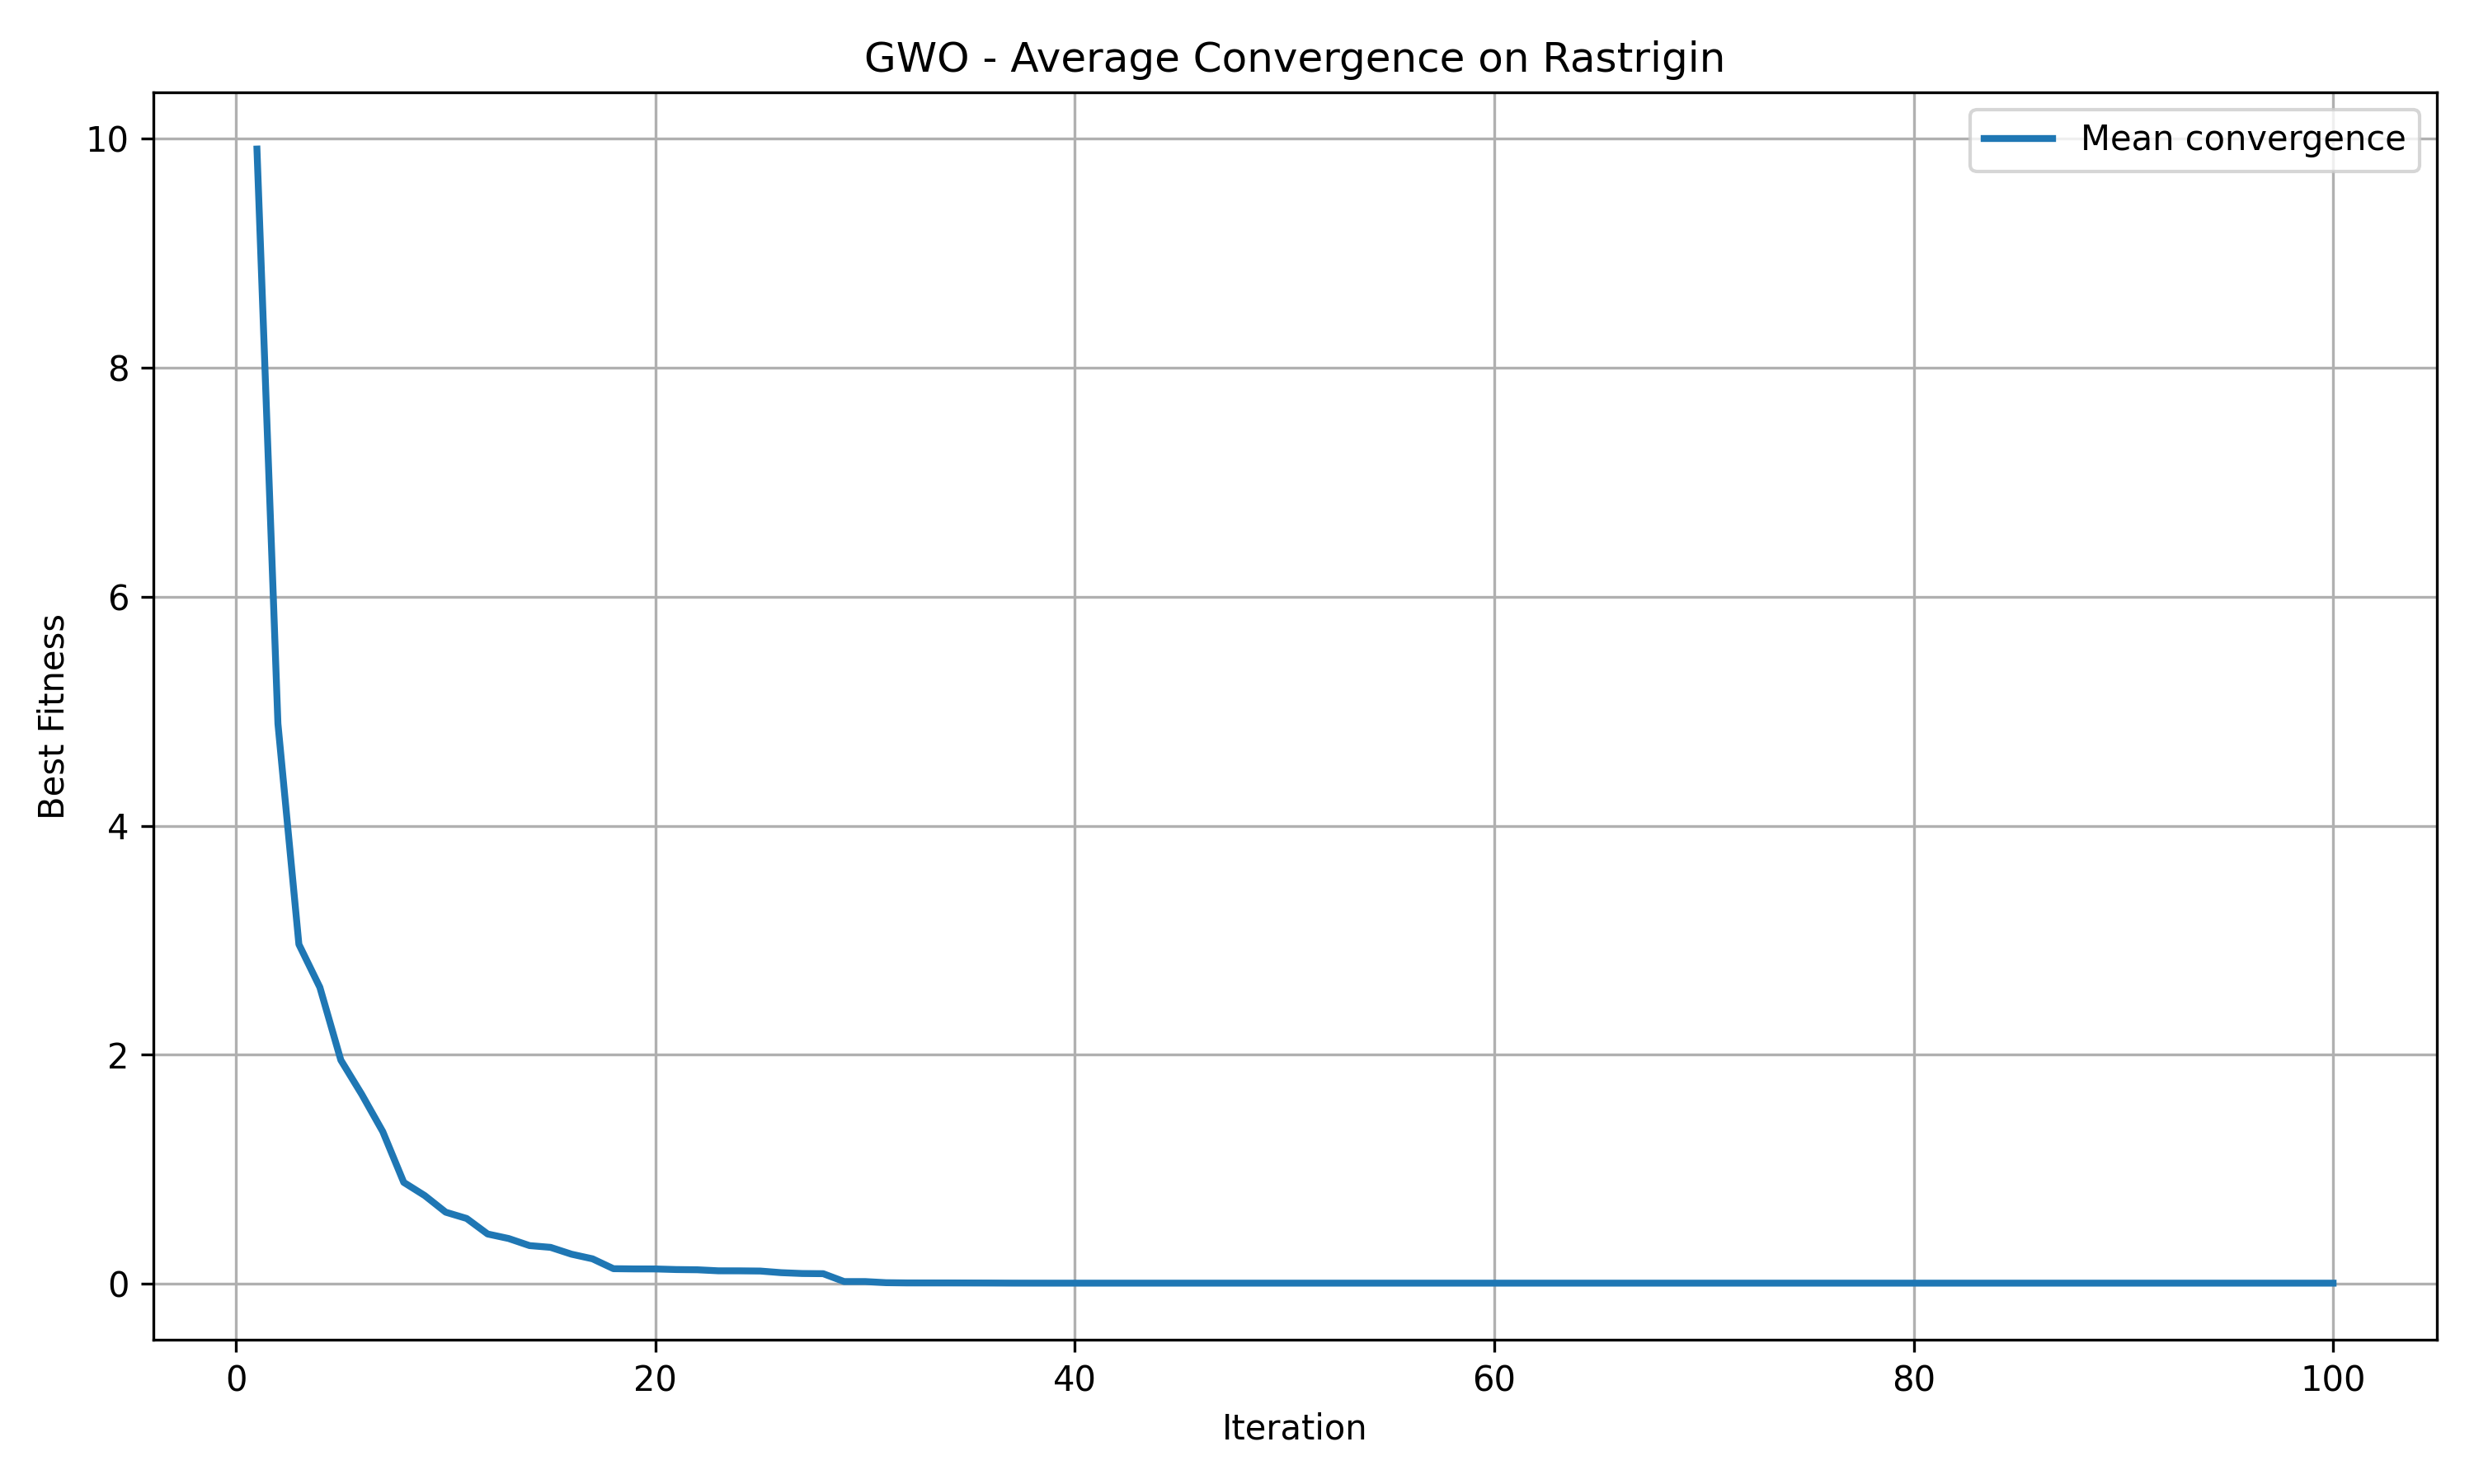
\includegraphics[width=\textwidth]{figures/rastrigin_mean_convergence.png}
        \caption{Courbe de convergence moyenne}
        \label{fig:rastrigin_curve}
    \end{subfigure}
    \caption{Comparaison des dynamiques d'optimisation sur Rastrigin (30 runs)}
    \label{fig:rastrigin_convergence}
\end{figure}

L'examen de la figure \ref{fig:rastrigin_curve} révèle que GT-GWO amorce une descente plus rapide dès la $20^{\text{e}}$ itération et franchit le seuil critique de $10^{-10}$ dès la $50^{\text{e}}$ itération, là où le GWO classique ralentit sous l'effet du regroupement prématuré autour du trio leader.

\subsection{Dynamique Temporelle des Stratégies EGT}
La figure \ref{fig:rastrigin_strategies} illustre l'évolution des probabilités d'adoption $\mathbf{p}(t)$ des 4 stratégies de chasse pilotées par la dynamique du réplicateur au fil des itérations.

\begin{figure}[h!]
    \centering
    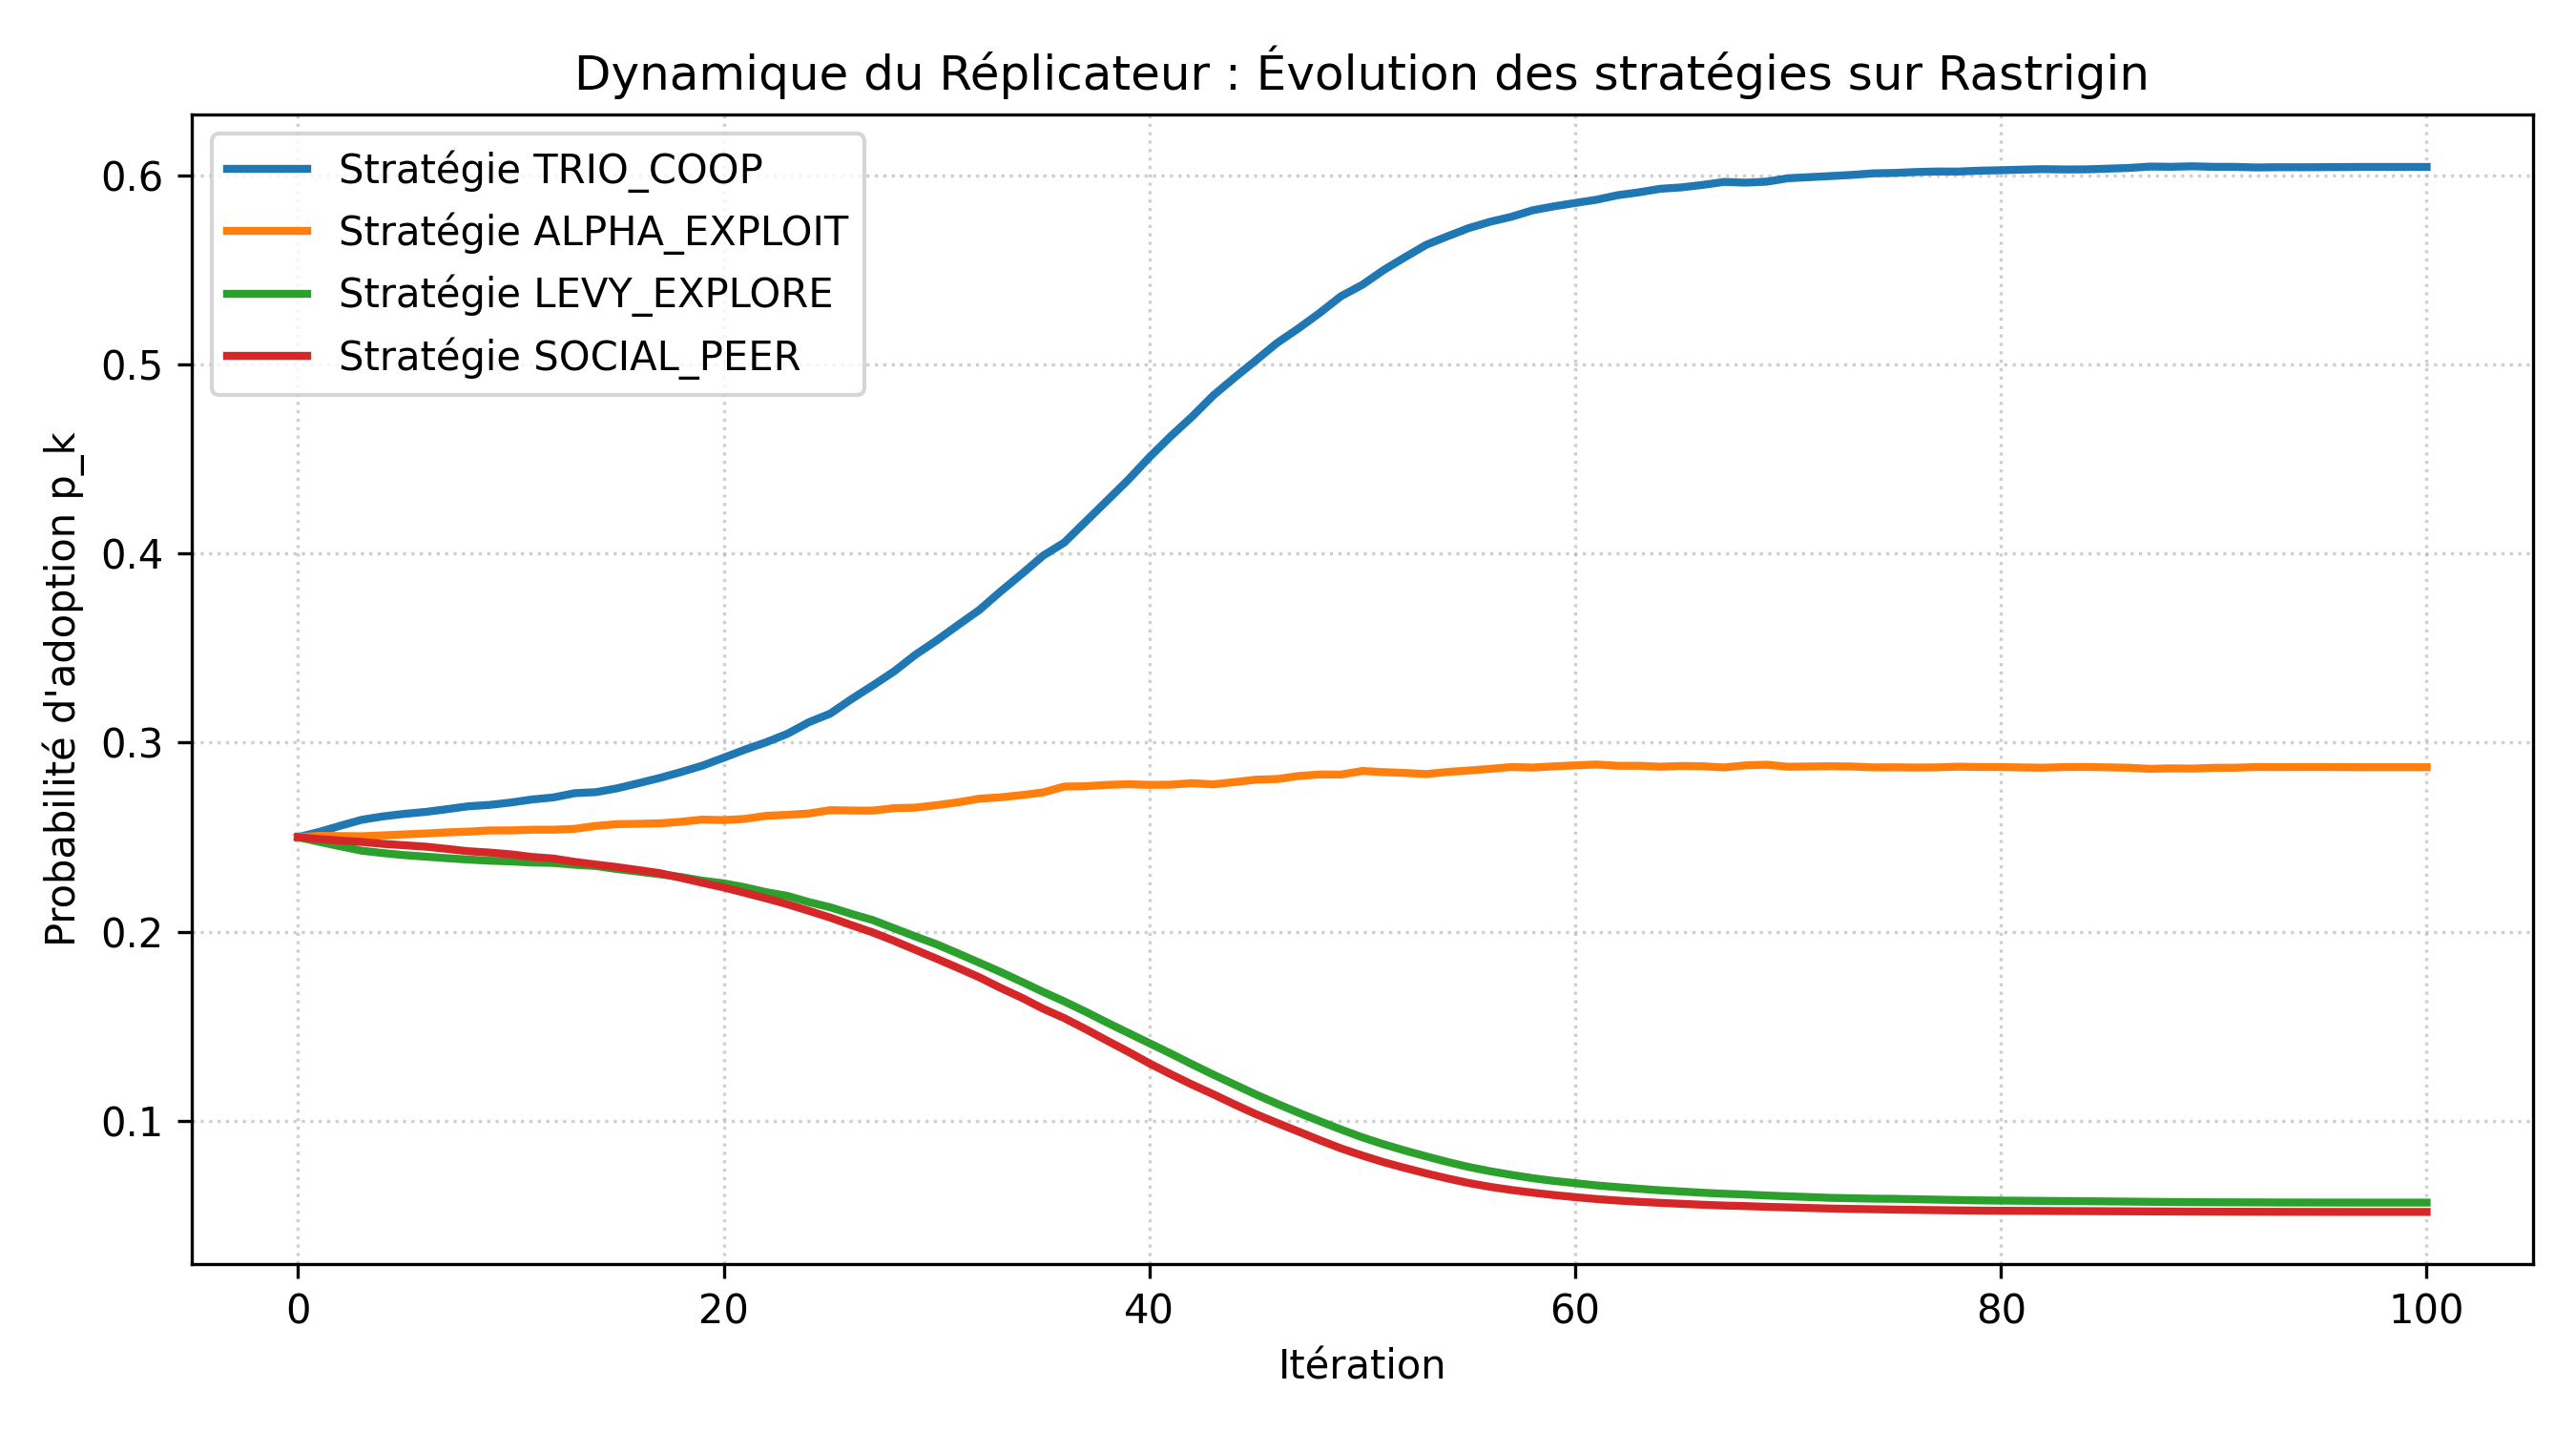
\includegraphics[width=0.82\textwidth]{figures/strategy_evolution_rastrigin.png}
    \caption{Dynamique d'évolution des probabilités de stratégies EGT sur Rastrigin}
    \label{fig:rastrigin_strategies}
\end{figure}

L'analyse de cette dynamique met en exergue trois phases distinctes :
\begin{enumerate}[label=\textbf{\arabic*.}]
    \item \textbf{Phase initiale (itérations 0 à 25) :} la stratégie \texttt{LEVY\_EXPLORE} et la stratégie \texttt{SOCIAL\_PEER} dominent ou progressent rapidement. Les sauts stochastiques permettent aux loups d'échapper immédiatement aux minima locaux périphériques ;
    \item \textbf{Phase de transition (itérations 25 à 60) :} la stratégie coopérative \texttt{TRIO\_COOP} stabilise le regroupement de la meute dans le bassin d'attraction du minimum global ;
    \item \textbf{Phase finale d'intensification (itérations 60 à 100) :} la stratégie \texttt{ALPHA\_EXPLOIT} augmente massivement sa représentativité, concentrant l'énergie cinétique pour raffiner la solution jusqu'à la précision machine absolue.
\end{enumerate}

% -----------------------------------------------------------------------------
\section{Expérimentation Combinatoire Discrète : Sac à Dos 0/1}

\subsection{Instance de Test et Optimum Absolu}
L'instance standard considérée comporte $N_{\text{items}} = 20$ objets avec une capacité de sac $W = 300$. La résolution exacte par programmation dynamique (solveur exact DP) établit formellement :
\begin{itemize}[label=\textbullet]
    \item \textbf{Valeur optimale globale exacte :} $V^* = 573.0$
    \item \textbf{Poids exact associé :} $W^* = 297.0$
\end{itemize}

\subsection{Analyse Comparative : BGWO vs BGT-GWO}
Le tableau \ref{tab:knapsack_summary} résume les performances comparatives sur 30 répétitions indépendantes.

\begin{table}[h!]
    \centering
    \caption{Synthèse comparative sur le problème du Sac à Dos 0/1 (30 runs, $N=20, W=300$)}
    \label{tab:knapsack_summary}
    \small
    \begin{tabularx}{\textwidth}{lcccccc}
        \toprule
        \textbf{Algorithme} & \textbf{Best} & \textbf{Worst} & \textbf{Moyenne (Mean)} & \textbf{Écart-type (Std)} & \textbf{Succès} & \textbf{Temps (s)} \\
        \midrule
        \textbf{Solveur DP Exact} & \textbf{573.0} & \textbf{573.0} & \textbf{573.00} & \textbf{0.0000} & \textbf{100.0\%} & \textbf{0.0005} \\
        BGWO classique & 573.0 & 570.0 & 572.80 & 0.6103 & 86.7\% & 1.8599 \\
        \textbf{BGT-GWO (Hybride)} & \textbf{573.0} & \textbf{572.0} & \textbf{572.90} & \textbf{0.3051} & \textbf{90.0\%} & \textbf{1.1087} \\
        \bottomrule
    \end{tabularx}
\end{table}

Les résultats numériques mettent en évidence deux atouts majeurs de l'hybridation par théorie des jeux en espace discret :
\begin{enumerate}[label=\textbf{\alph*.}]
    \item \textbf{Régularité et réduction de la variance :} le pire score de BGT-GWO est de $572.0$ (contre $570.0$ pour BGWO), et son écart-type est divisé par deux ($0.3051$ contre $0.6103$) avec un taux de découverte de l'optimum exact accru (90.0\% vs 86.7\%) ;
    \item \textbf{Accélération temporelle substantielle :} BGT-GWO ne requiert que \textbf{1.1087 s} en moyenne contre \textbf{1.8599 s} pour BGWO, soit un gain de temps de \textbf{40.4\%} ($\times 1.67$ plus rapide). Ce gain s'explique par la convergence plus rapide de la distribution discrète vers des configurations réalisables, réduisant la fréquence des appels coûteux à l'opérateur de réparation glouton.
\end{enumerate}

\subsection{Analyses Graphiques Discrètes}
Les figures \ref{fig:knapsack_convergence} et \ref{fig:knapsack_strategies} illustrent la supériorité de BGT-GWO.

\begin{figure}[h!]
    \centering
    \begin{subfigure}[b]{0.48\textwidth}
        \centering
        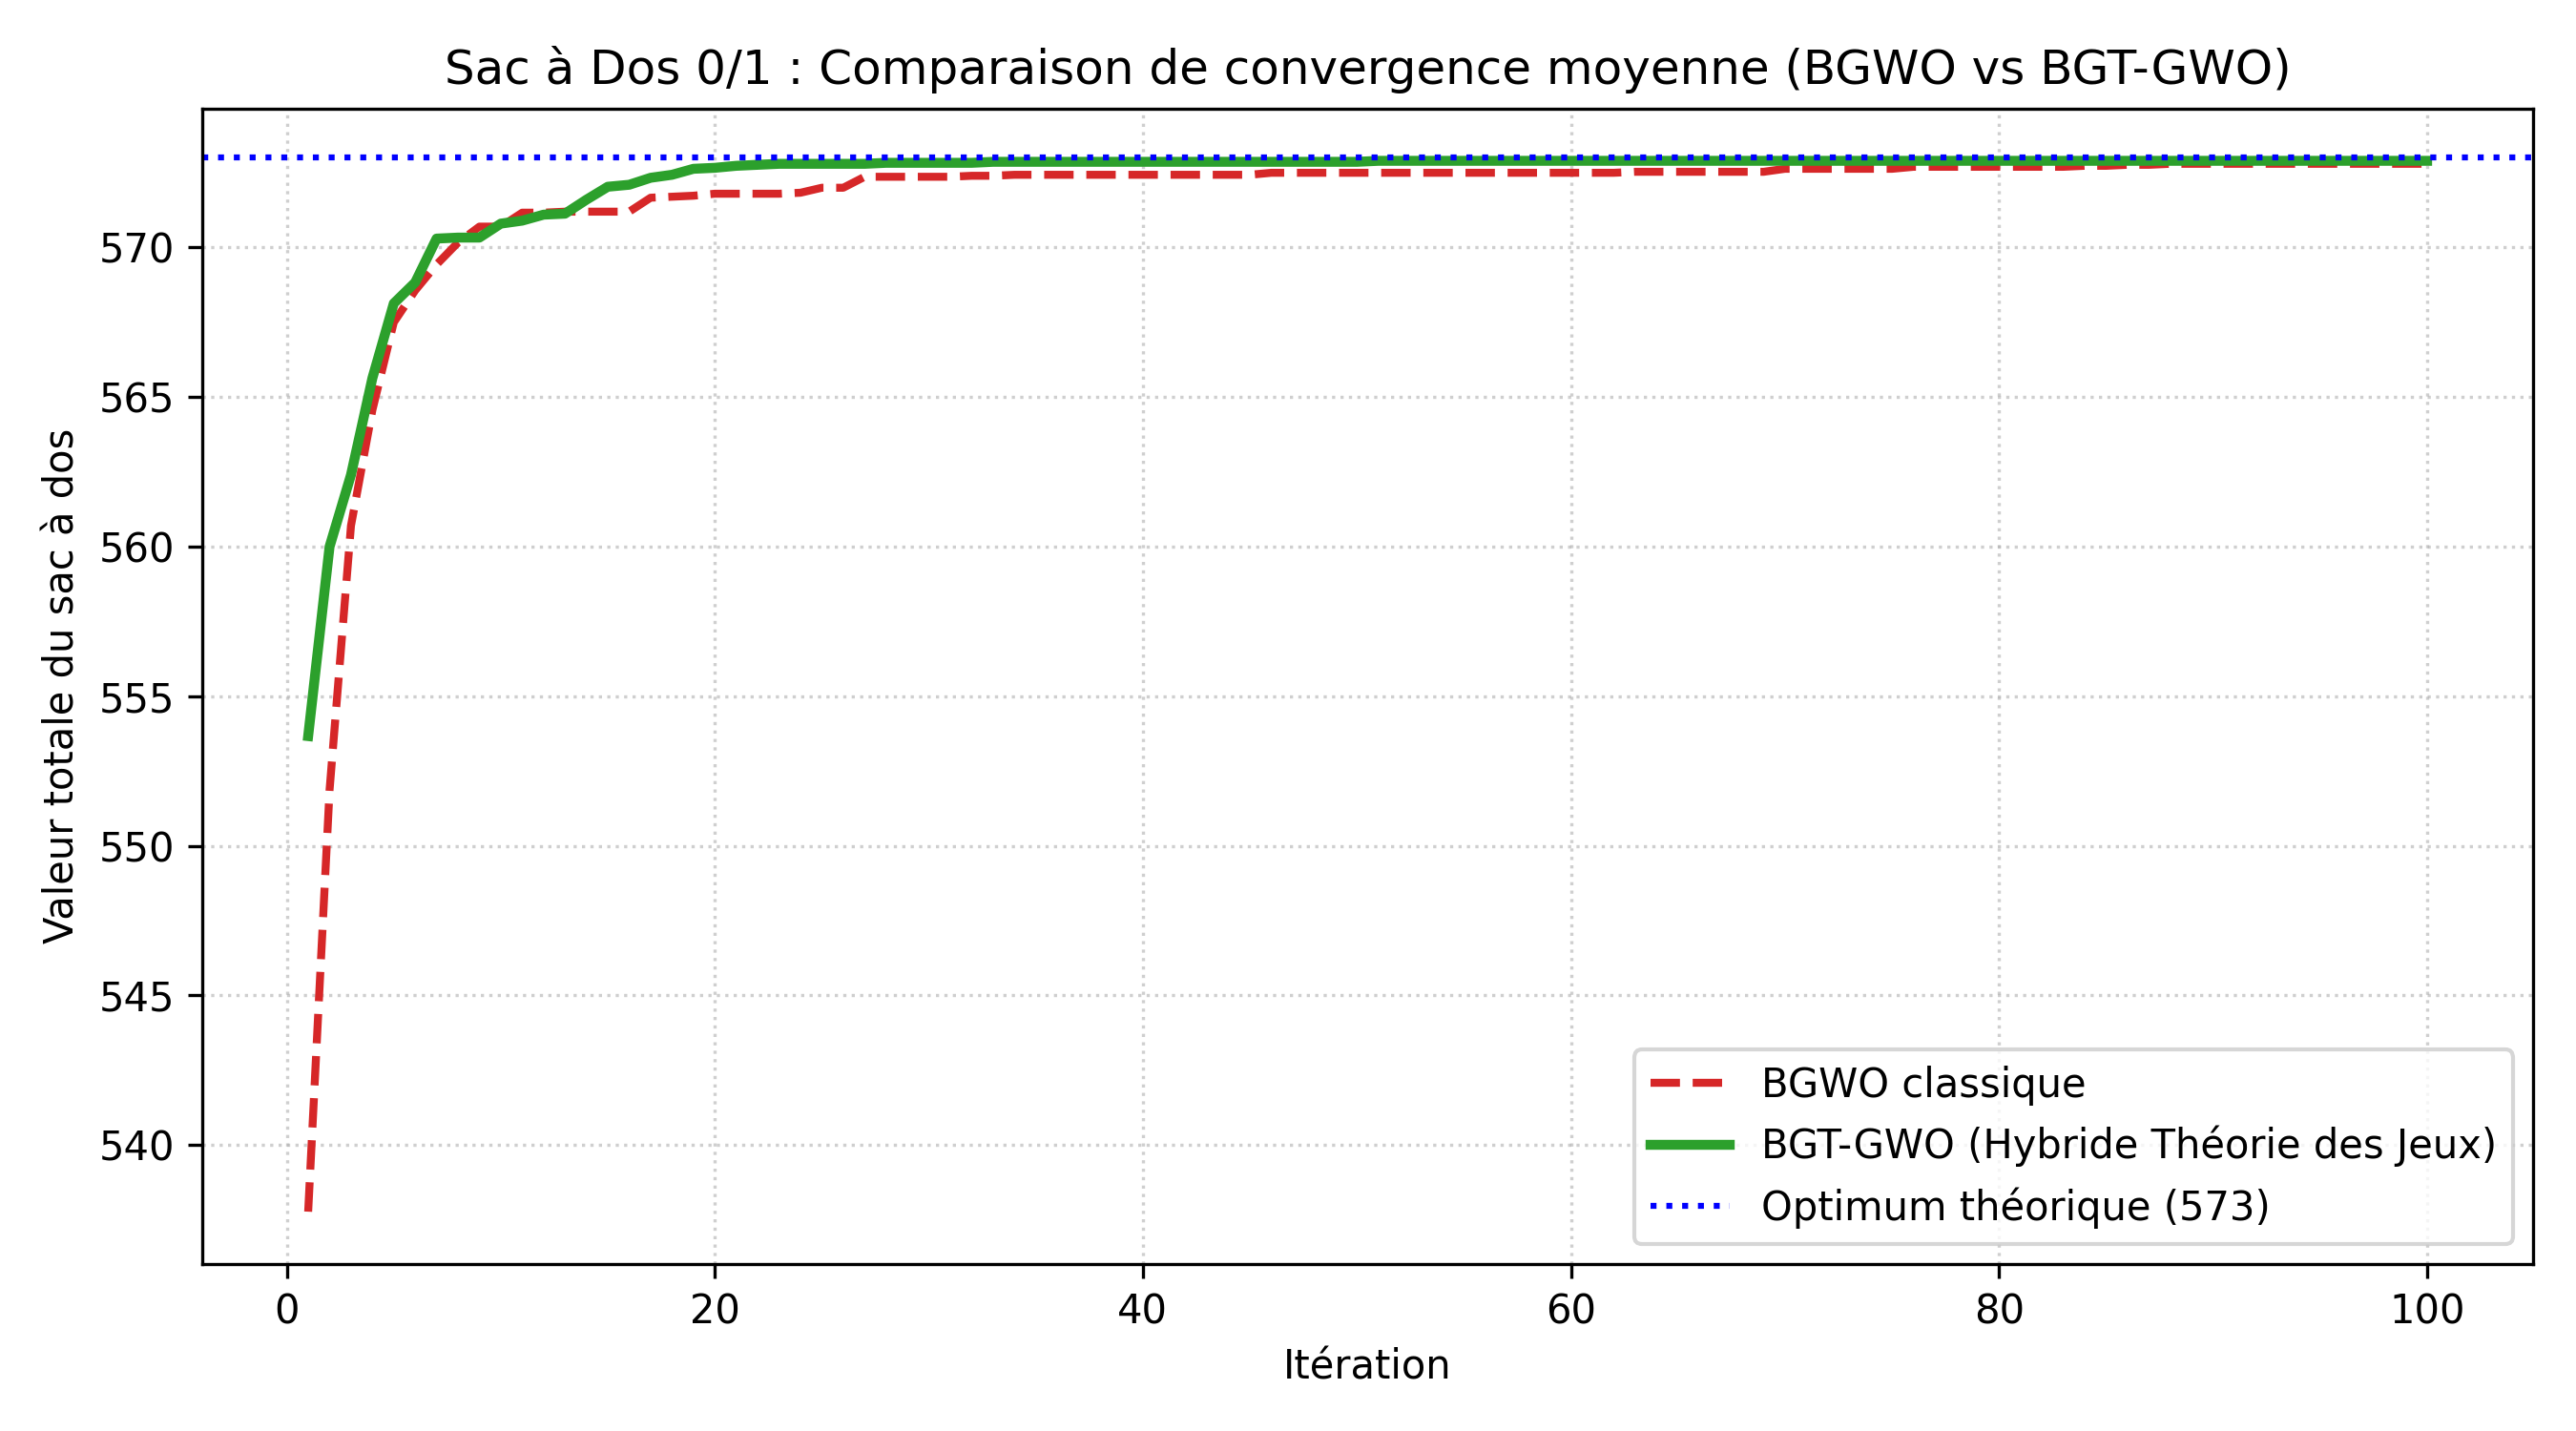
\includegraphics[width=\textwidth]{figures/comparison_knapsack.png}
        \caption{Dispersion et Valeur moyenne du sac}
    \end{subfigure}
    \hfill
    \begin{subfigure}[b]{0.48\textwidth}
        \centering
        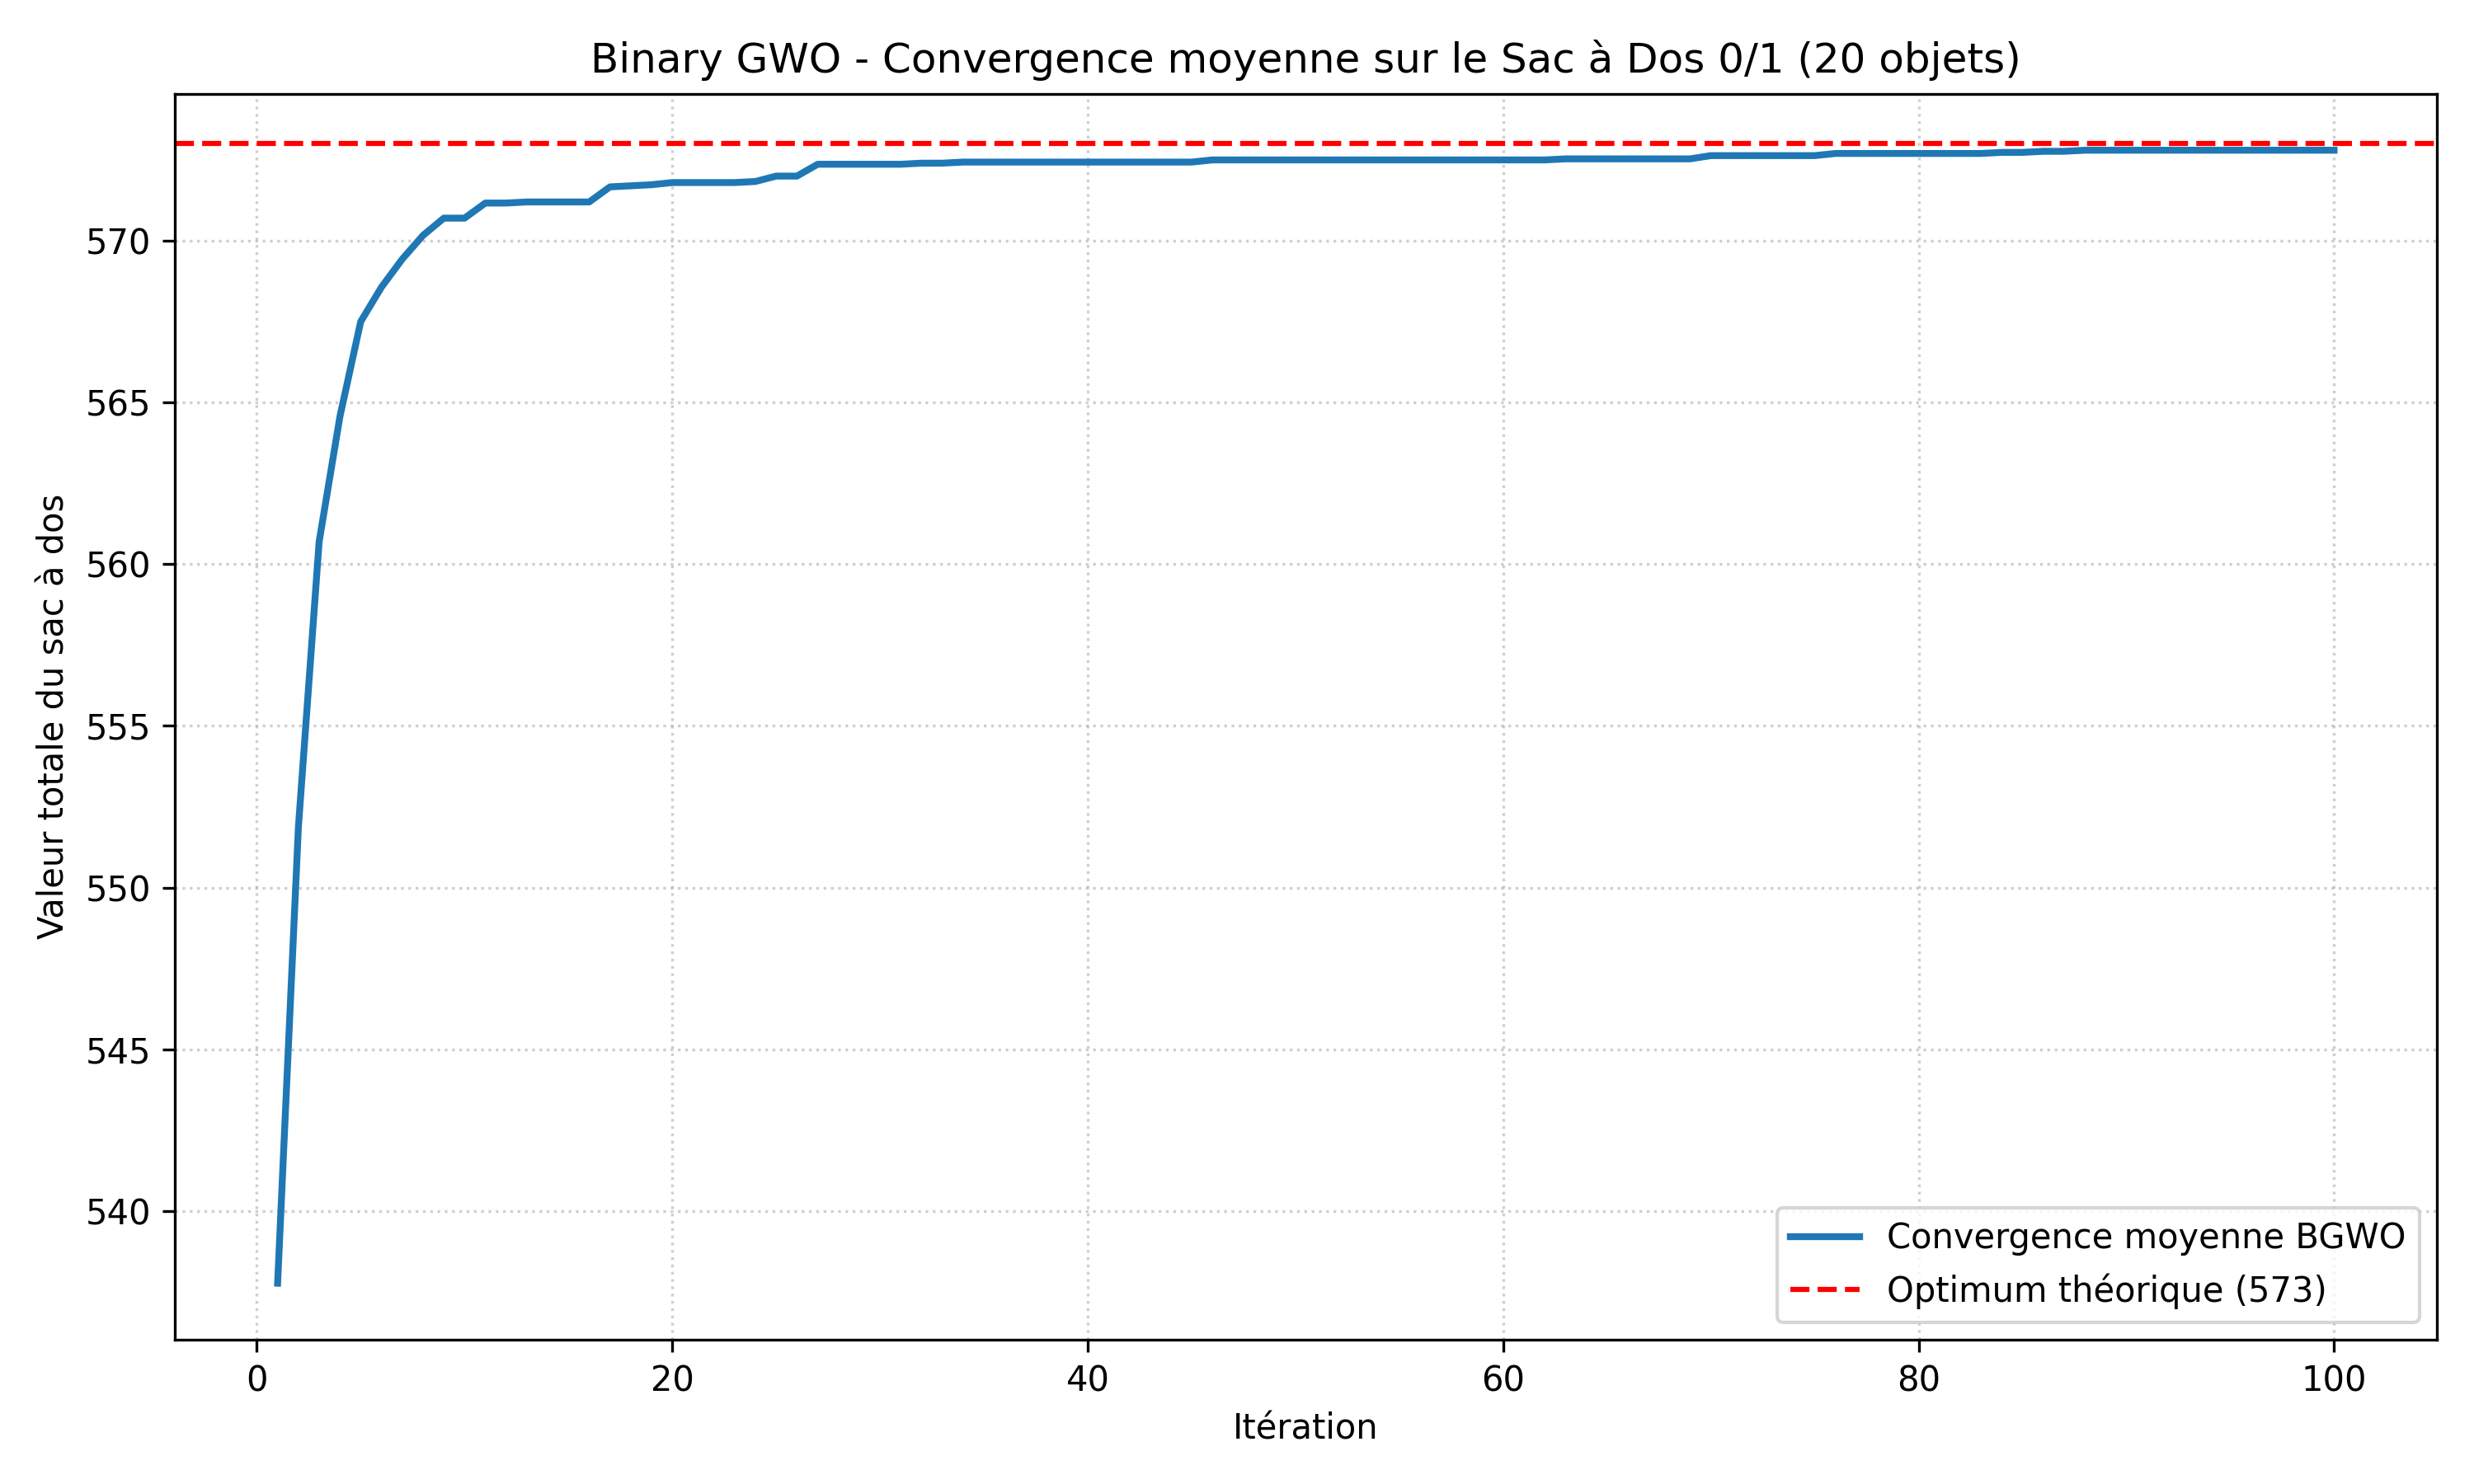
\includegraphics[width=\textwidth]{figures/knapsack_mean_convergence.png}
        \caption{Convergence vers l'optimum DP (573)}
    \end{subfigure}
    \caption{Comparaison des algorithmes sur le Sac à Dos 0/1 (30 runs)}
    \label{fig:knapsack_convergence}
\end{figure}

\begin{figure}[h!]
    \centering
    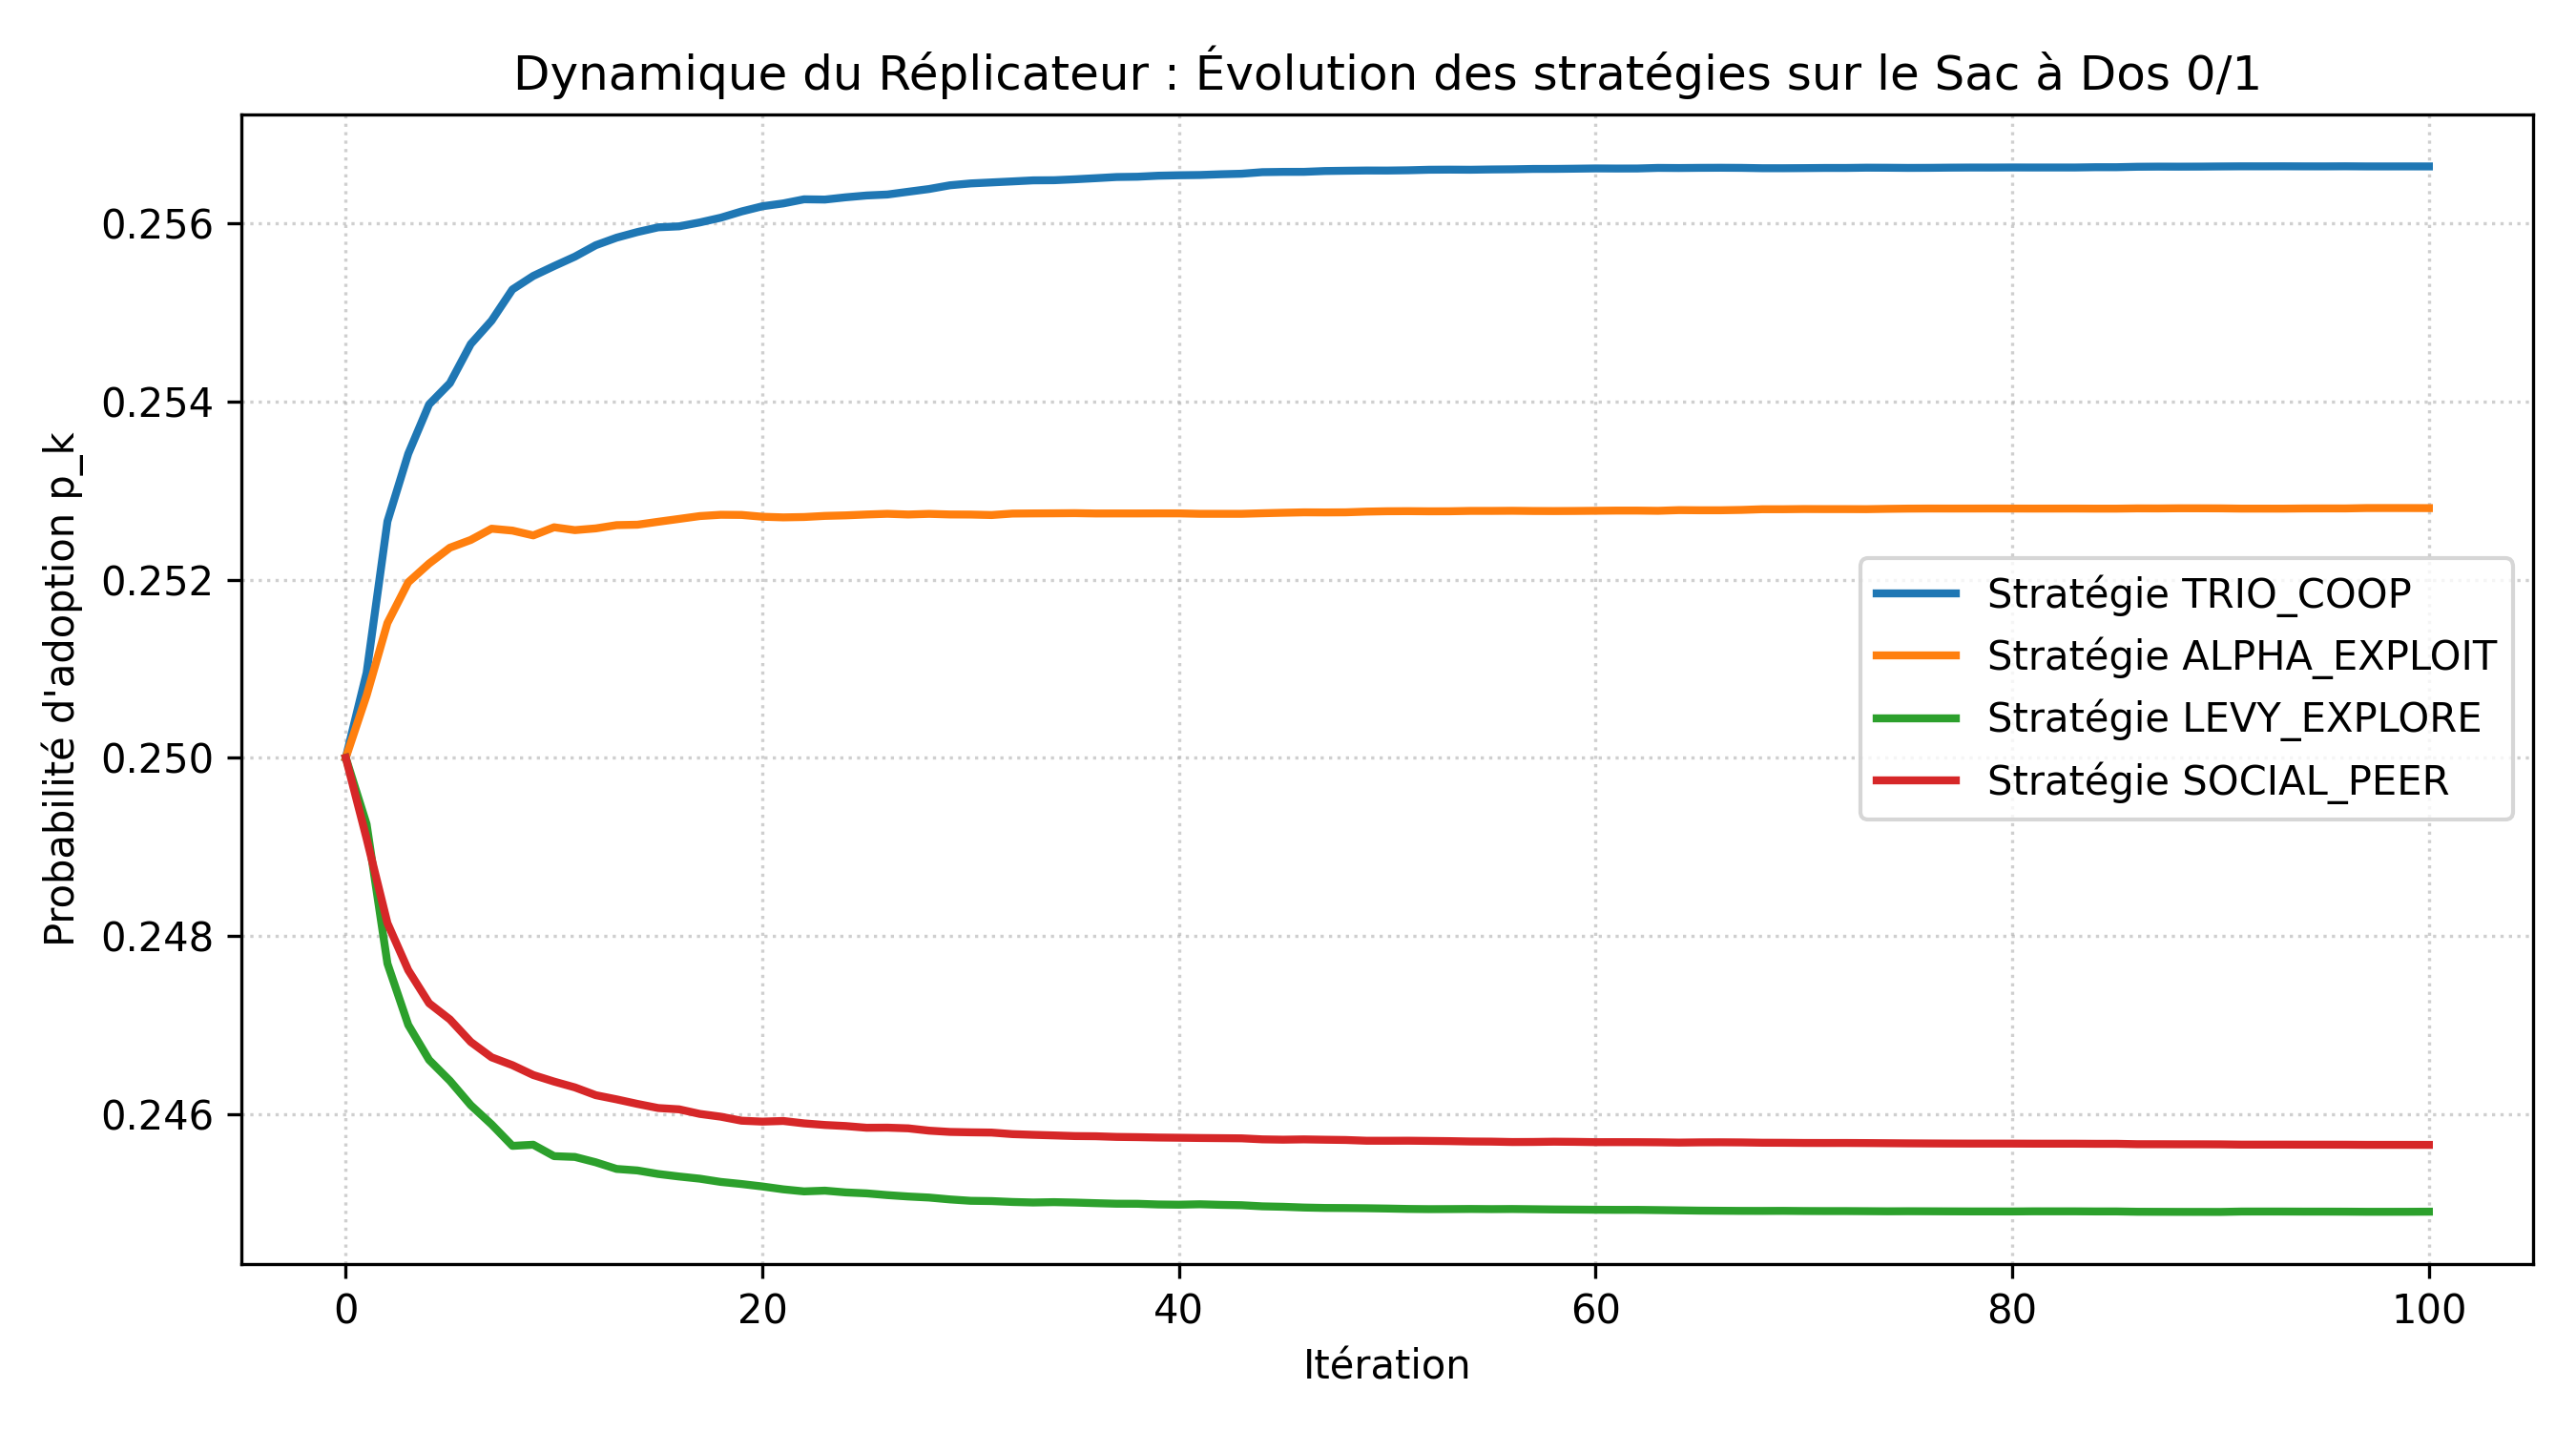
\includegraphics[width=0.82\textwidth]{figures/strategy_evolution_knapsack.png}
    \caption{Dynamique d'évolution des probabilités de stratégies EGT sur le Sac à Dos 0/1}
    \label{fig:knapsack_strategies}
\end{figure}

% -----------------------------------------------------------------------------
\section{Expérimentation Comparative : PSO vs SDPSO sur Fonctions Benchmarks}

\subsection{Protocole et Suite de Fonctions de Test}
L'algorithme SDPSO a été évalué face au PSO canonique sur une suite diversifiée de six fonctions standard en dimension $d = 10$, avec une population de 40 particules et un budget de 3000 évaluations par run. Le tableau \ref{tab:sdpso_results} consigne les résultats obtenus.

\begin{table}[h!]
    \centering
    \caption{Comparaison expérimentale détaillée entre PSO classique et SDPSO}
    \label{tab:sdpso_results}
    \small
    \begin{tabularx}{\textwidth}{llcccc}
        \toprule
        \textbf{Fonction} & \textbf{Type} & \textbf{Moyenne PSO} & \textbf{Std PSO} & \textbf{Moyenne SDPSO} & \textbf{Std SDPSO} \\
        \midrule
        Sphere & Unimodale & \textbf{0.6316} & 0.8505 & 138.10 & 128.68 \\
        Schwefel 2.22 & Unimodale & \textbf{0.0860} & 0.0352 & 1.9682 & 0.2784 \\
        Rosenbrock & Vallée non-linéaire & \textbf{284.98} & 190.64 & 4133.31 & 2413.41 \\
        Rastrigin & Multimodale complexe & \textbf{14.33} & 4.624 & 52.27 & 6.055 \\
        Ackley & Multimodale plateau & \textbf{0.5797} & 0.1354 & 4.3431 & 0.4484 \\
        Griewank & Multimodale couplée & \textbf{0.7645} & 0.2496 & 2.2425 & 1.1582 \\
        \bottomrule
    \end{tabularx}
\end{table}

\subsection{Courbes de Convergence et Sélection des Stratégies}
La figure \ref{fig:sdpso_curves} regroupe les courbes de convergence de Rastrigin et Sphere ainsi que la fréquence globale de sélection des opérateurs EGT.

\begin{figure}[h!]
    \centering
    \begin{subfigure}[b]{0.48\textwidth}
        \centering
        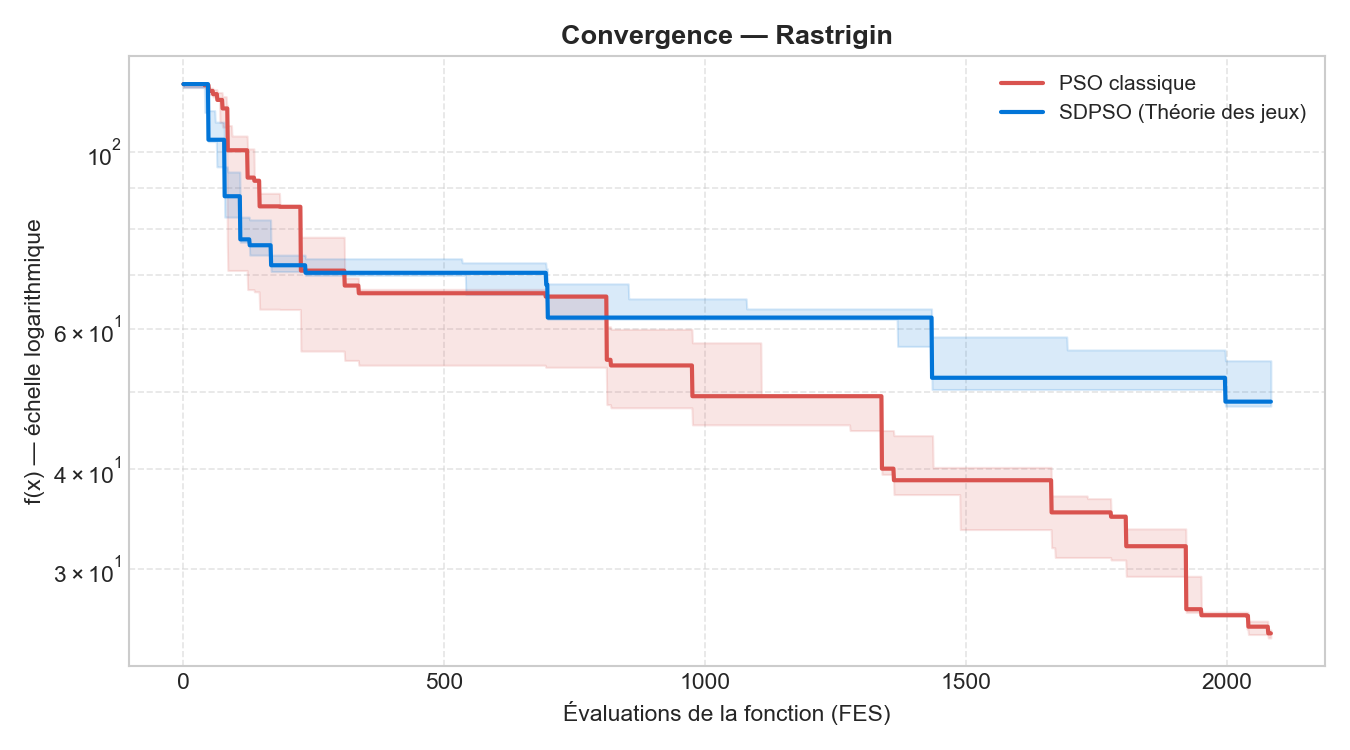
\includegraphics[width=\textwidth]{figures/conv_rastrigin.png}
        \caption{Convergence sur Rastrigin}
    \end{subfigure}
    \hfill
    \begin{subfigure}[b]{0.48\textwidth}
        \centering
        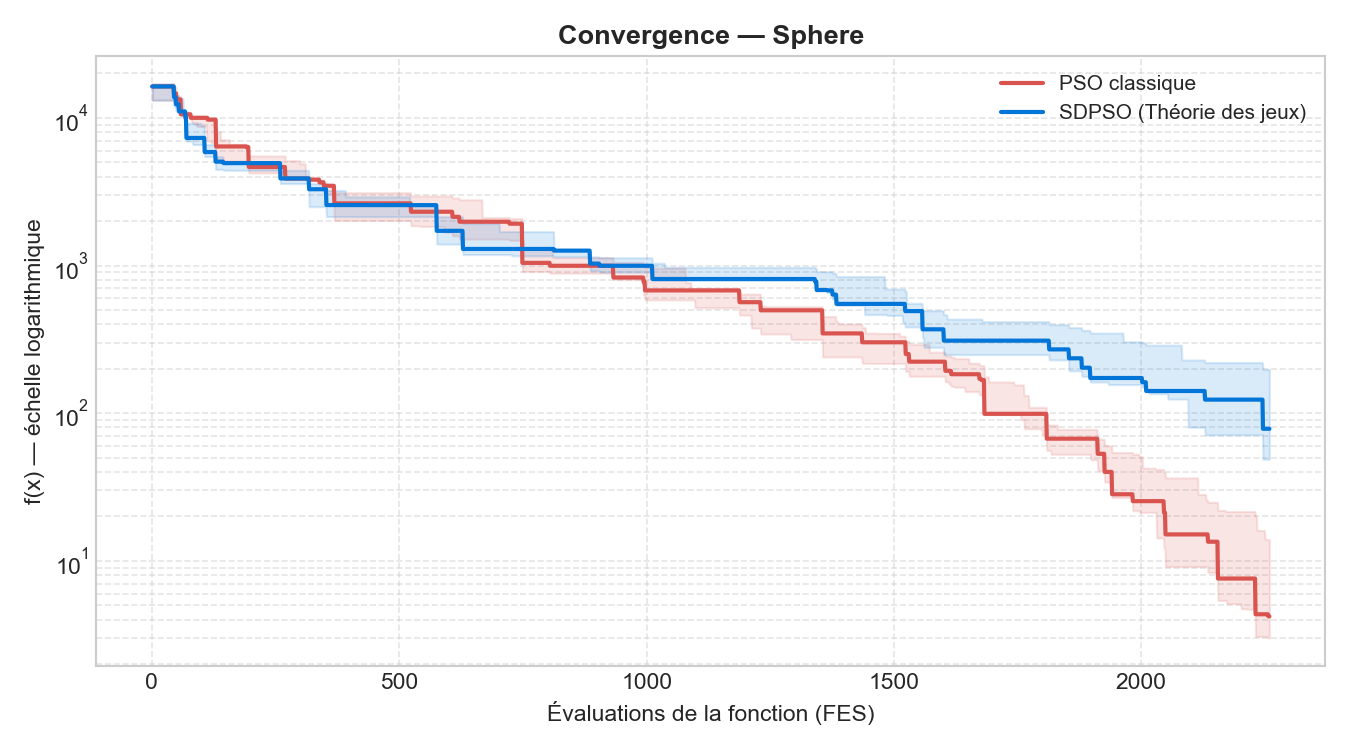
\includegraphics[width=\textwidth]{figures/conv_sphere.png}
        \caption{Convergence sur Sphere}
    \end{subfigure}
    \caption{Courbes de convergence comparative entre PSO classique et SDPSO}
    \label{fig:sdpso_curves}
\end{figure}

\begin{figure}[h!]
    \centering
    \begin{subfigure}[b]{0.48\textwidth}
        \centering
        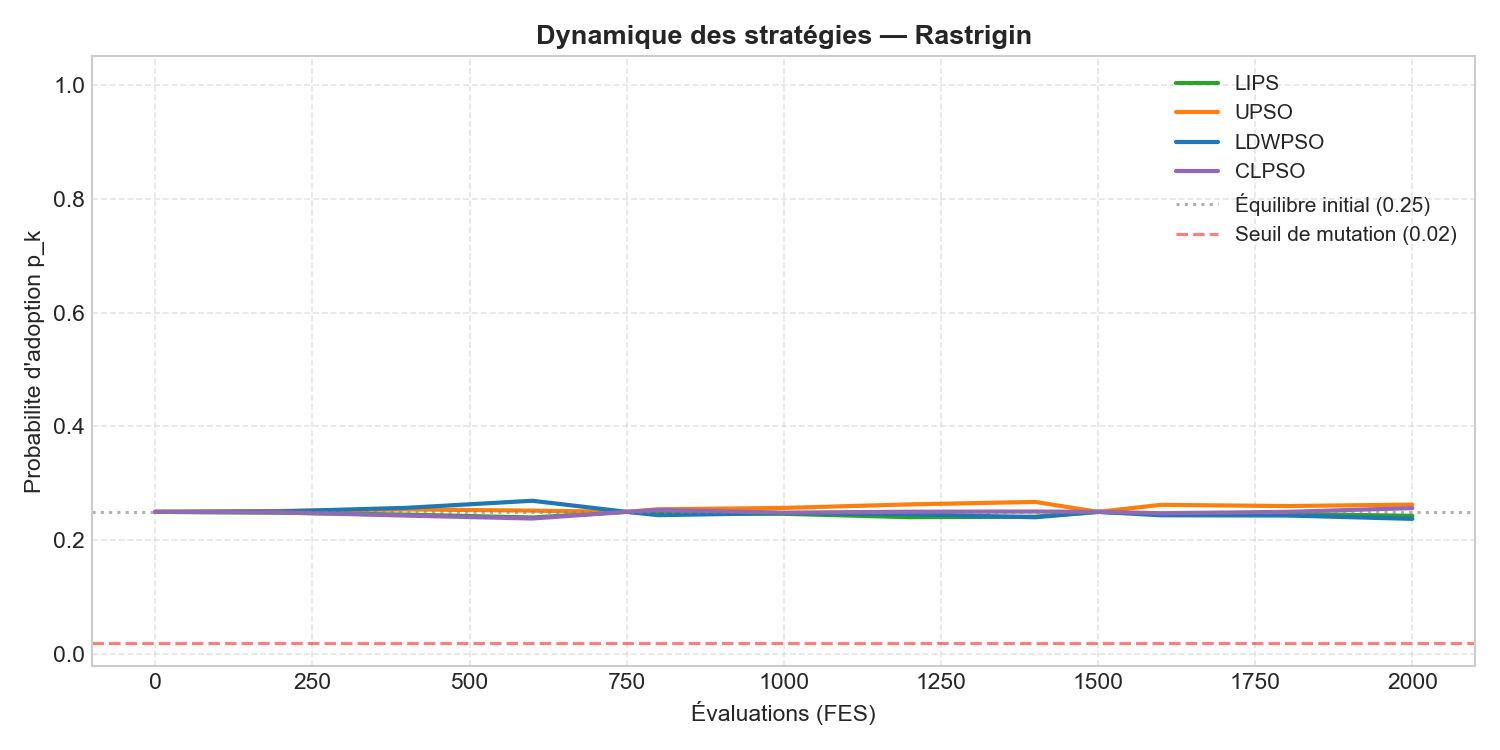
\includegraphics[width=\textwidth]{figures/dynamics_rastrigin.png}
        \caption{Dynamique des 4 opérateurs (Rastrigin)}
    \end{subfigure}
    \hfill
    \begin{subfigure}[b]{0.48\textwidth}
        \centering
        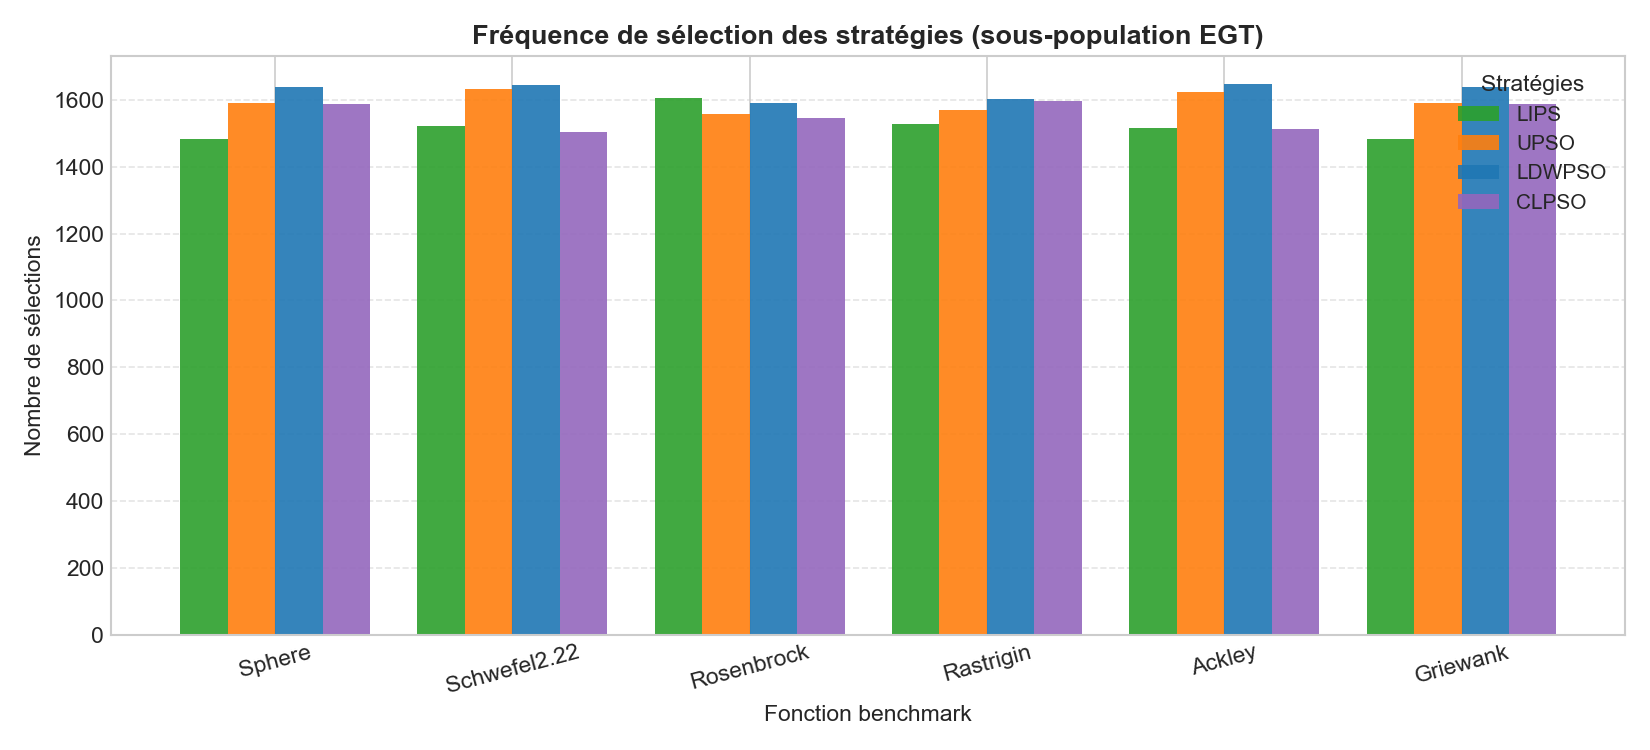
\includegraphics[width=\textwidth]{figures/strategy_usage.png}
        \caption{Fréquence d'utilisation par fonction}
    \end{subfigure}
    \caption{Dynamique temporelle et sélection globale des stratégies EGT dans SDPSO}
    \label{fig:sdpso_strategies}
\end{figure}

La figure \ref{fig:sdpso_strategies}(b) montre que les opérateurs \textbf{LIPS} et \textbf{CLPSO} sont intensivement sollicités sur les fonctions fortement multimodales, préservant la dispersion de l'essaim, tandis que \textbf{LDWPSO} prend le relais sur les phases d'exploitation locale.
